\documentclass[spanish,12pt,a4paper,titlepage]{report}
\usepackage[utf8]{inputenc}
\usepackage{graphicx}
\usepackage{subfig}
\usepackage{float}
\usepackage{wrapfig}
\usepackage{multirow}
\usepackage{caption}
\usepackage[spanish]{babel}
\usepackage[dvips]{hyperref}
\usepackage{amssymb}
\usepackage{listings}
\usepackage{epsfig}
\usepackage{amsmath}
\usepackage{array}
\usepackage[table]{xcolor}
\usepackage{multirow}
%\usepackage[Sonny]{fncychap}
\usepackage[Lenny]{fncychap}
%\usepackage[Glenn]{fncychap}
%\usepackage[Conny]{fncychap}
%\usepackage[Rejne]{fncychap}
%\usepackage[Bjarne]{fncychap}
%\usepackage[Bjornstrup]{fncychap}

%\usepackage{subfiles}
%\usepackage{framed}

\setlength{\topmargin}{-1.5cm}
\setlength{\textheight}{25cm}
\setlength{\oddsidemargin}{0.3cm} 
\setlength{\textwidth}{15cm}
\setlength{\columnsep}{0cm}

\newcommand{\degc}{$^\circ$C}

\begin{document}

\chapter{Barómetro}
\label{chap:barometro}

Al analizar la performance del GPS como medio para determinar la elevación del cuadricóptero, se determinó que sería problemático, principalemente por la baja frecuencia de muestreo del GPS, y por la baja precisión de los datos obtenidos.
\begin{itemize}
\item Se obtiene un valor para la altura absoluta, libre de bias, pero hace falta promediar muestras durante varios minutos antes de llegar a un datos confiable.
\item  La precisión del GPS es mala muy cerca del suelo, lo cual representa un problema al intentar despegar y/o aterrizar.
\end{itemize}

Se optó por incorporar un barómetro, ya que aparentemente dichos senores padecen de \textit{otros} problemas, y pueden complementar al GPS.

Se trata de un barómetro digital BOSCH BMP085. Permite medir presión absoluta, y, conociendo la presión y la temperatura a nivel del mar, permite calcular la altura absoluta.

Puede trabajar en varios modos. Existe un compromiso entre el consumo, la tasa de actualización, y la resolución, y dicho compromiso se especifica al elegir el modo de funcionamiento.

\section{Objetivos}
%\ref{} agregar refs

El objetivo de estas pruebas es determinar como se usará el barómetro BOSCH BMP085, incorporado para asistir en la determinación de la altura del cuadricóptero. Para ello se procede a caracterizar el sensor.

Se analizan las siguientes situaciones:

\begin{itemize}
\item Reposo: Se analizaron períodos del orden de:
  \begin{itemize}
  \item Decenas de minutos: Caracterizar el drift y el tiempo de \textit{warm-up}.
  \item Decenas de segundos: Caracterización del ruido de las medidas.
  \end{itemize}
\item Altura relativa: 3 experimentos variando el rango a analizar.
  \begin{itemize}
  \item Puntos que distan decenas de centímetros entre sí.
  \item Puntos que distan 1m entre sí.
  \item Puntos que distan aproximadamente 5m entre sí.
  \end{itemize}
\end{itemize}

\newpage
\section{Materiales}
\label{sec:materiales}

\begin{itemize}
\item Laptop.
\item Tanza.
\item Cinta métrica.
\item Cubo de lapacho.
\item IMU ``Mongoose'' de CKDevices, con un BMP085.
\end{itemize}

\section{Consideraciones previas}
\label{consideraciones}

A nivel de la tropósfera, la capa más baja de la atmósfera, se puede calcular la altura a partir de la presión atmosférica mediante la siguiente fórmula\cite{bib:alt-press}:

\begin{equation}
  \label{eq:press-alt}
  p = p_0 \cdot \left(1 - \frac{L \cdot h}{T_0} \right)^\frac{g \cdot M}{R \cdot L}
\end{equation}

Donde:
\begin{itemize}
\item p0: 	Presión atmosférica estándar a nivel del mar -	101325 Pa
\item L :	Gradiente de temperatura\footnote{Tasa de incremento de la temperatura con la altura (es negativa).} -	0.0065 K/m
\item T0:	Temperatura estándar a nivel del mar -	288.15 K
\item g :	Constante de gravitación universal -	9.80665 m/s2
\item M :	Masa molar del aire seco -	0.0289644 kg/mol
\item R :	Constante universal de los gases - 	8.31447 J/(mol$\cdot$K)
\end{itemize}


\newpage
\section{Procedimiento}
\label{sec:procedimiento}

\subsection{Drift y \textit{warm-up}}
\label{sec:drift-y-warm-up}

Observando datos, se notó lo que parecería ser un drift en las medidas obtenidas del barómetros. Se tomarán muestras durante 1 hora, con el barómetro quieto, comenzando con el circuito en frío\footnote{Habiendo estado apagado durante, por lo menos, los 30 minutos previos a la prueba.}.

\subsection{Caracterización del ruido}

Es de interés caracterizar el ruido en los datos provenientes del barómetro. Si se trata de un proceso estacionario, y de ruido blanco, entonces, promediando se pueden obtener datos más exactos.

Se analizan datos tomados durante diversos períodos de tiempo: 5 minutos, 2 minutos, 20 segundos y 15 segundos.

Se analiza la autocorrelación de las muestras, y se compara el ruído con los valores dados por la hoja de datos. La hoja de datos especifica ruído RMS típico para los distintos modos de funcionamiento

\subsection{Medidas de altura absoluta}

Para analizar la performance del barómetro como instrumento para determinar la elevación absoluta, se toman puntos de altura conocida, y se comparan las lecturas contra los datos conocidos.

\subsection{Distancias de varios metros}

Se deja despliega una cinta métrica en el vacío del centro de una escalera de 4 tramos en la Facultad de Ingeniería de la Universidad de la República. La cinta extendida cubre aproximadamente 25 metros. Se comparan las medidas dadas por el barómetro con las que se obtienen de la cinta.

Se utiliza una cinta de agrimensor, graduada cada 10 centímetros.

\vspace{-20pt}
\begin{figure}[H]
  \begin{center}
	\subfloat[Toma de datos.]{\label{fig:escalera_compu.jpg}
	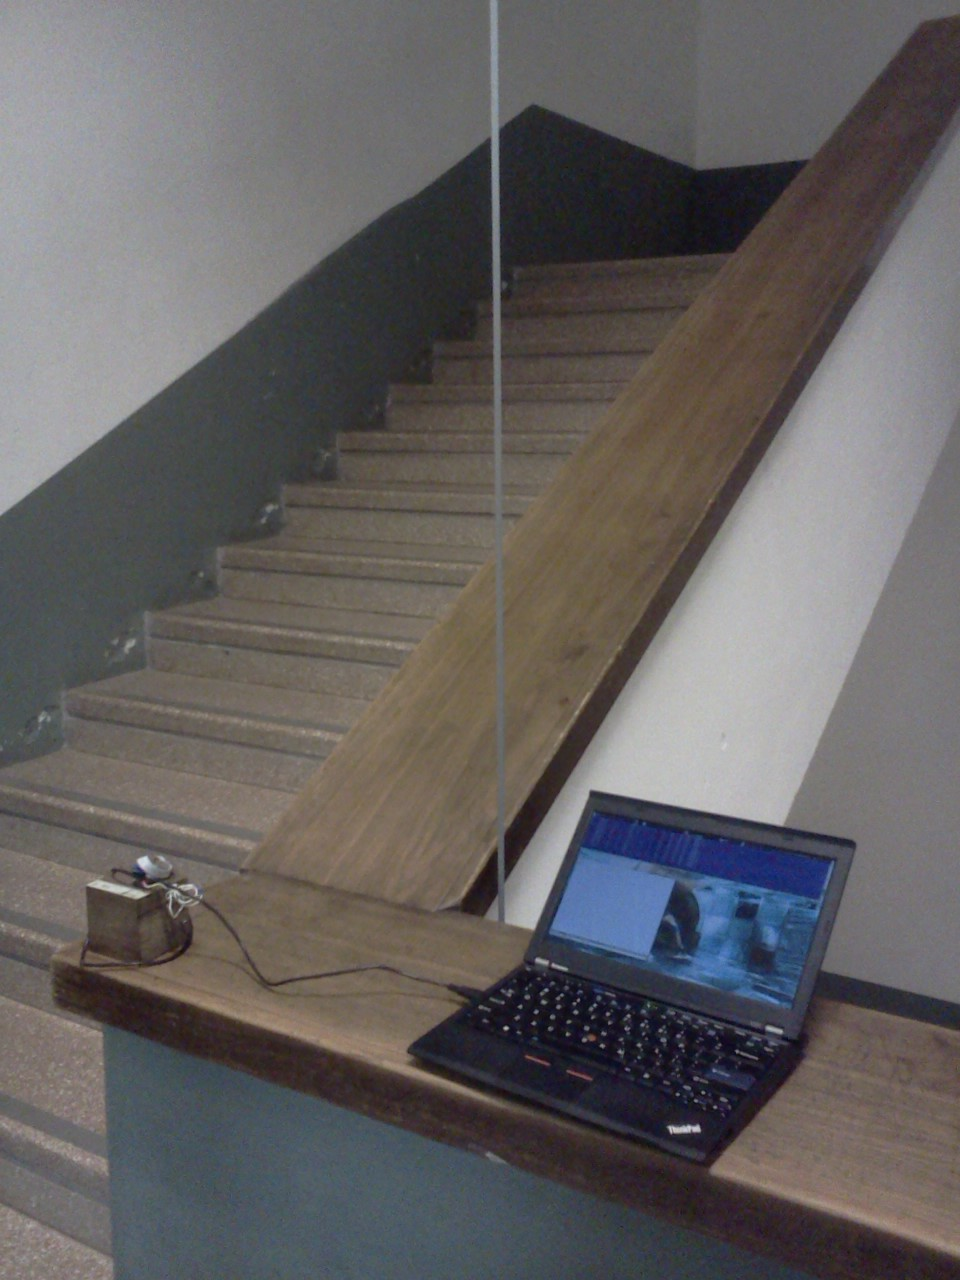
\includegraphics[width=0.35\textwidth]
		{./pics/escalera_compu.jpg}}
	\subfloat[Vacío de la escalera.]{\label{fig:escalera_pater.jpg}
	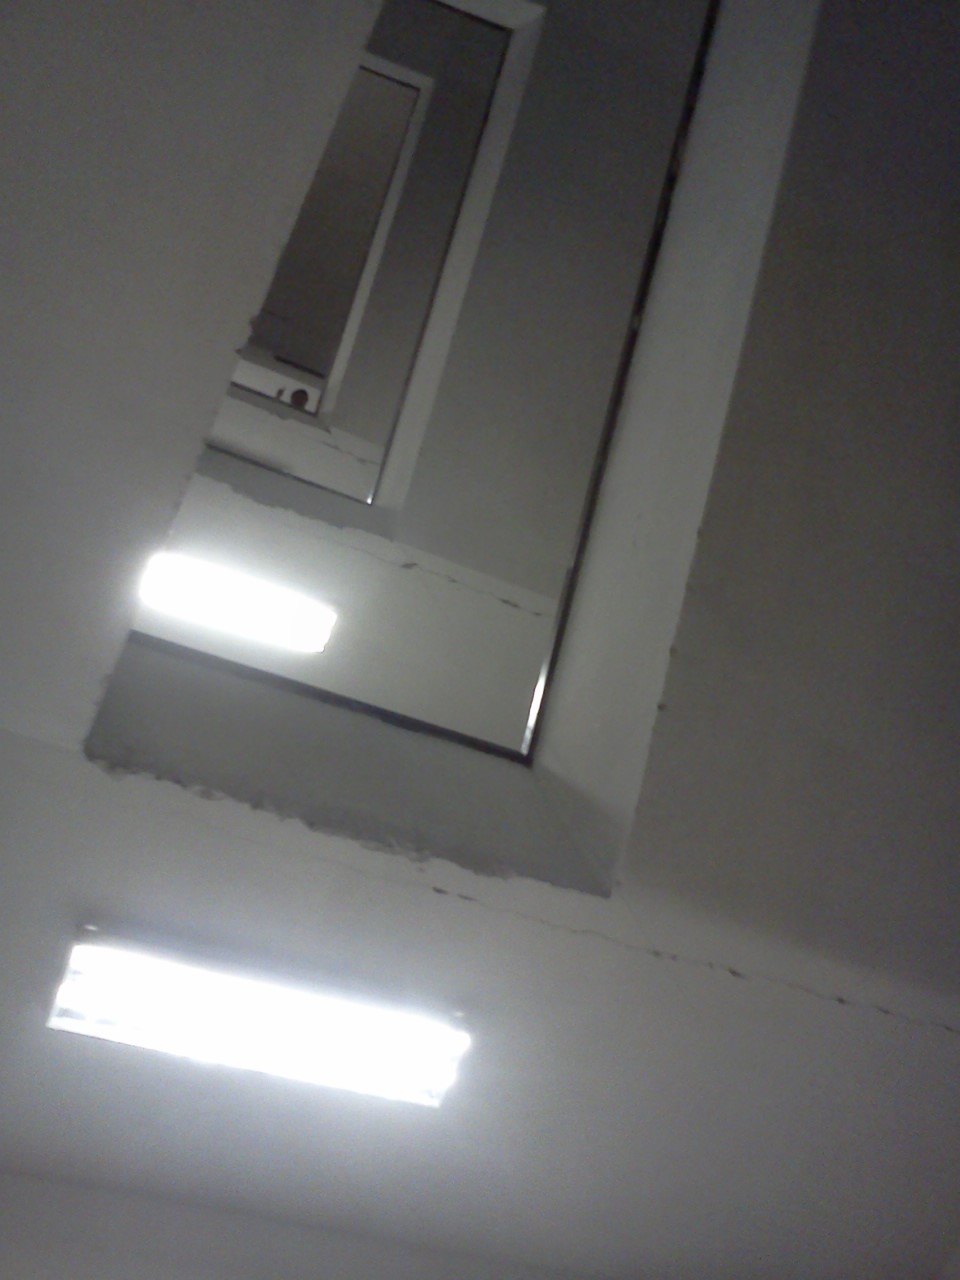
\includegraphics[width=0.35\textwidth]
		{./pics/escalera_pater.jpg}}
  \end{center}
\vspace{-20pt}
  \caption{Experimento: Distancias de varios metros.}
\label{fig:escalera-fing}
\end{figure}

\subsection{Distancias de un metro}

Se toma una tanza de algunos metros de longitud. Se realizan marcas cada un metro, en seis puntos distintos de la tanza. En un extremo de la tanza se ata el cubo de lapacho, con la \emph{Mongoose} atornillada a el. Se lo deja bajar desde la escalera del \emph{IMERL}\footnote{Instituto de Matemática y Estadística Rafael Laguarda}. Se suelta tanza hasta que el cubo se apoye contra el piso, de forma que la primer marca en la cuerda se encuentre junto a quien está realizando las medidas. Se hace una pequeña marca sobre la baranda, en el punto que coincide con la primer marca de la cuerda. Se toma la medida de presión durante un minuto. Luego se sube el cubo hasta que la marca en la baranda coincida con la segunda marca de la cuerda (1 metro más arriba). Se vuelve a tomar la medida de presión. Se repite el procedimiento hasta tener la medida de presión en 5 alturas distintas. 
Se repite el experimento dos veces. Luego se toma la medida de presión a nivel del suelo. Se toman medidas mientras se sube y se baja el barómetro dos veces, se vuelven a tomar medidas a nivel del suelo.
\subsection{Distancias de decenas de centímetros}

Se ubica el cubo de lapacho siempre en la misma orientación sobre cada uno de los estantes de una estantería. Se coloca el cubo sobre el primer estante. Se mide la altura desde el suelo a la cara del cubo sobre la cual se encuentra apoyada la IMU. Se mide la presión durante un minuto. Se mueve el cubo al estante siguiente. Se vuelve a medir la altura respecto del suelo con un metro y se toman las medidas de presión durante un minuto. Se repite el procedimiento para los seis estantes que componen la estantería. 

\newpage
\section{Análisis y resultados}

\subsection{Drift y \textit{warm-up}}
\label{sec:drift-y-warm-up}

Para observar si hay un drift y/o tiempo de \textit{warm-up} significativo, se procedió a tomar muestras durante 1 hora, habiendo estado el dispositivo desenchufado durante por lo menos media hora (circuito arranca en frio).

Se repitió este experimento varias veces. En las figuras \ref{fig:1hora_01.pdf} y \ref{fig:1hora_01.pdf} se observan los resultados característicos.

\begin{figure}[h!]
  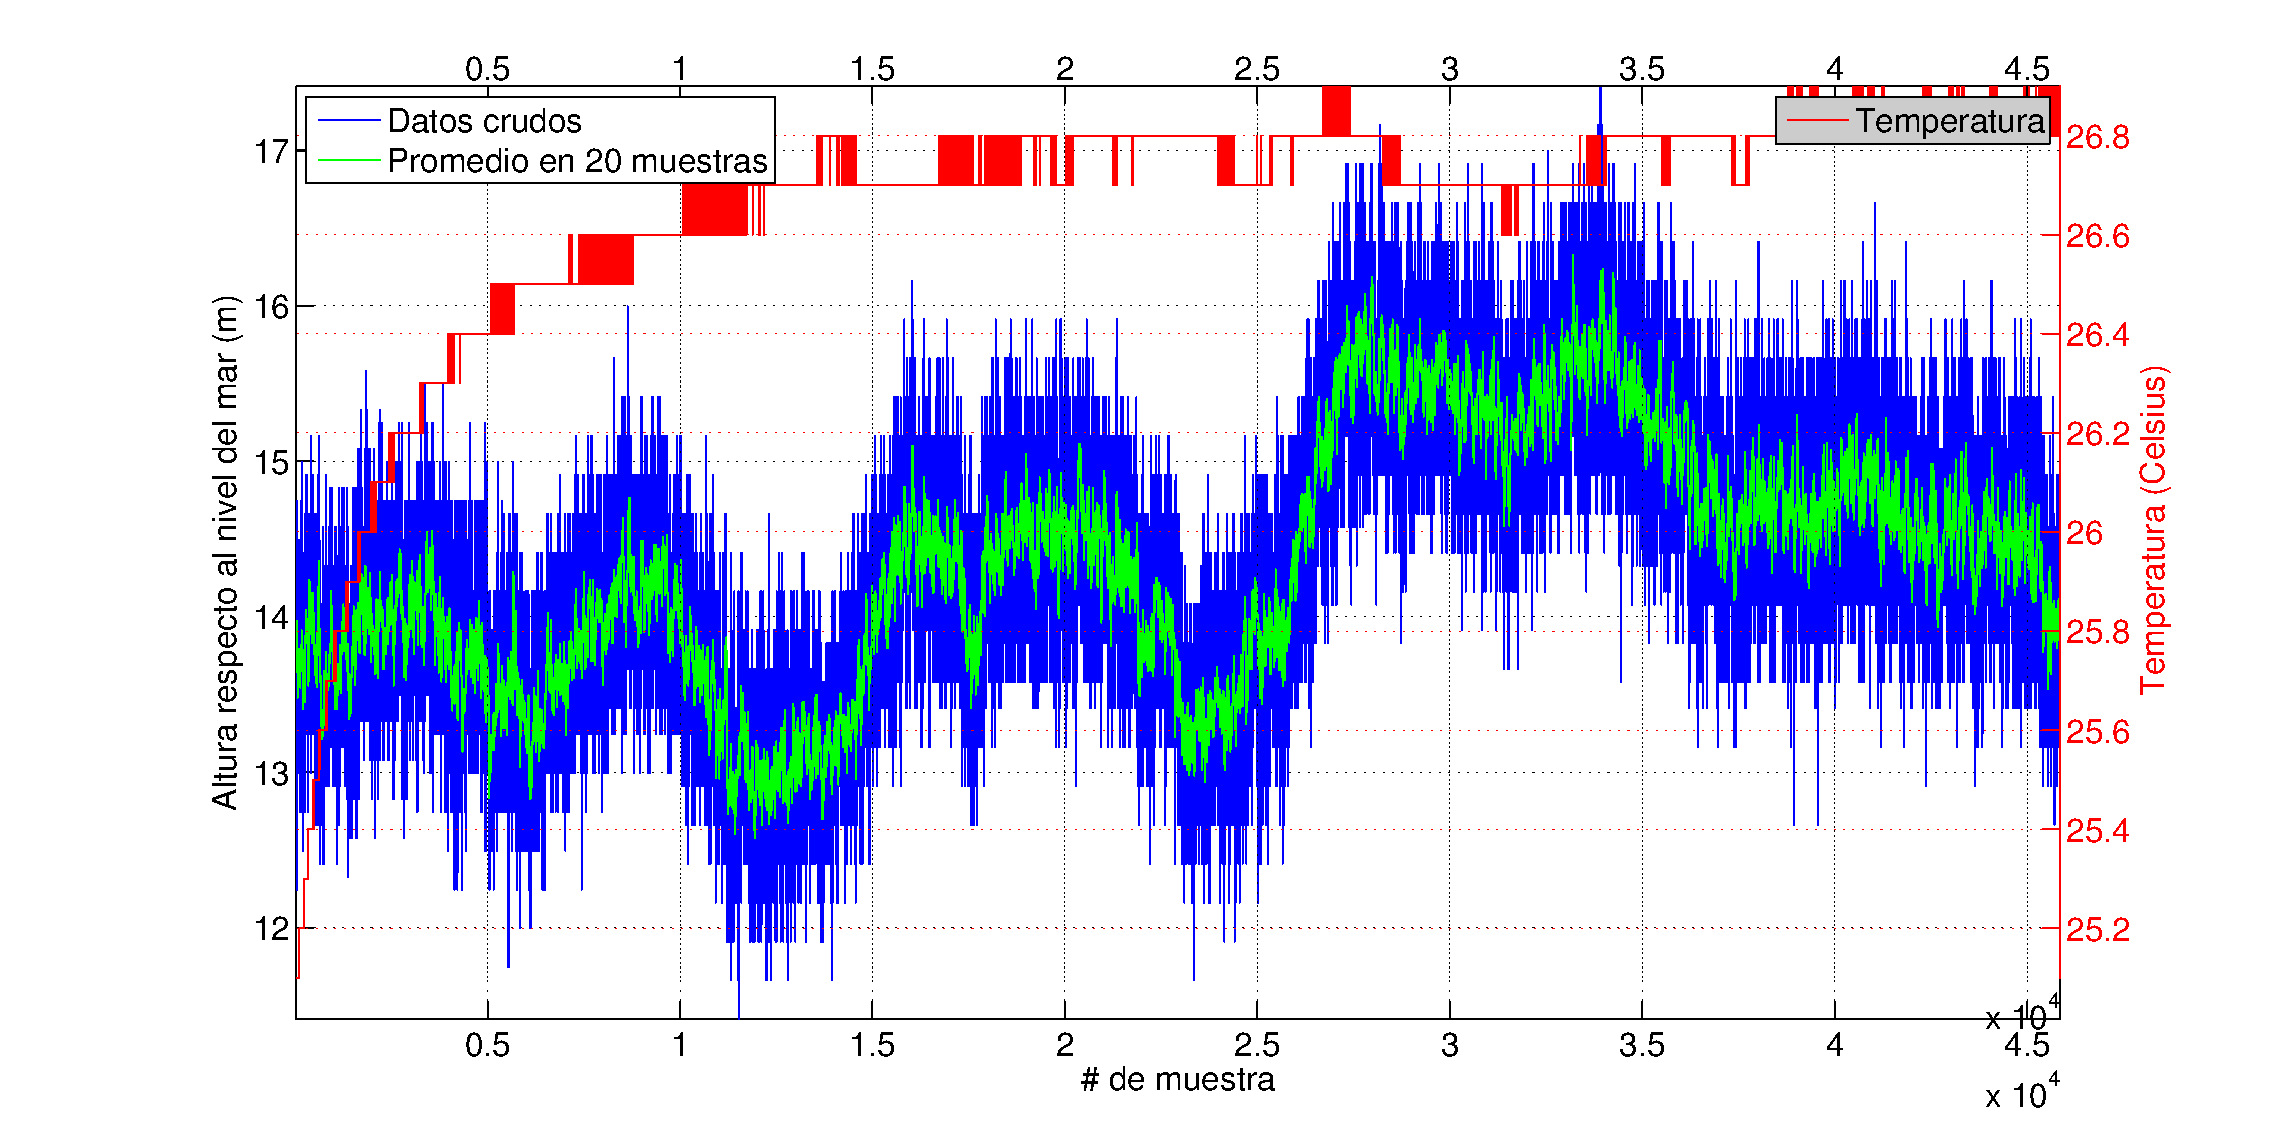
\includegraphics[width=.9\textwidth]{./pics/1hora_04.pdf}
  \caption{Muestras durante una hora, experimento \#4.}
  \label{fig:1hora_04.pdf}
\end{figure}
\vspace{-20pt}
\begin{figure}[h!]
  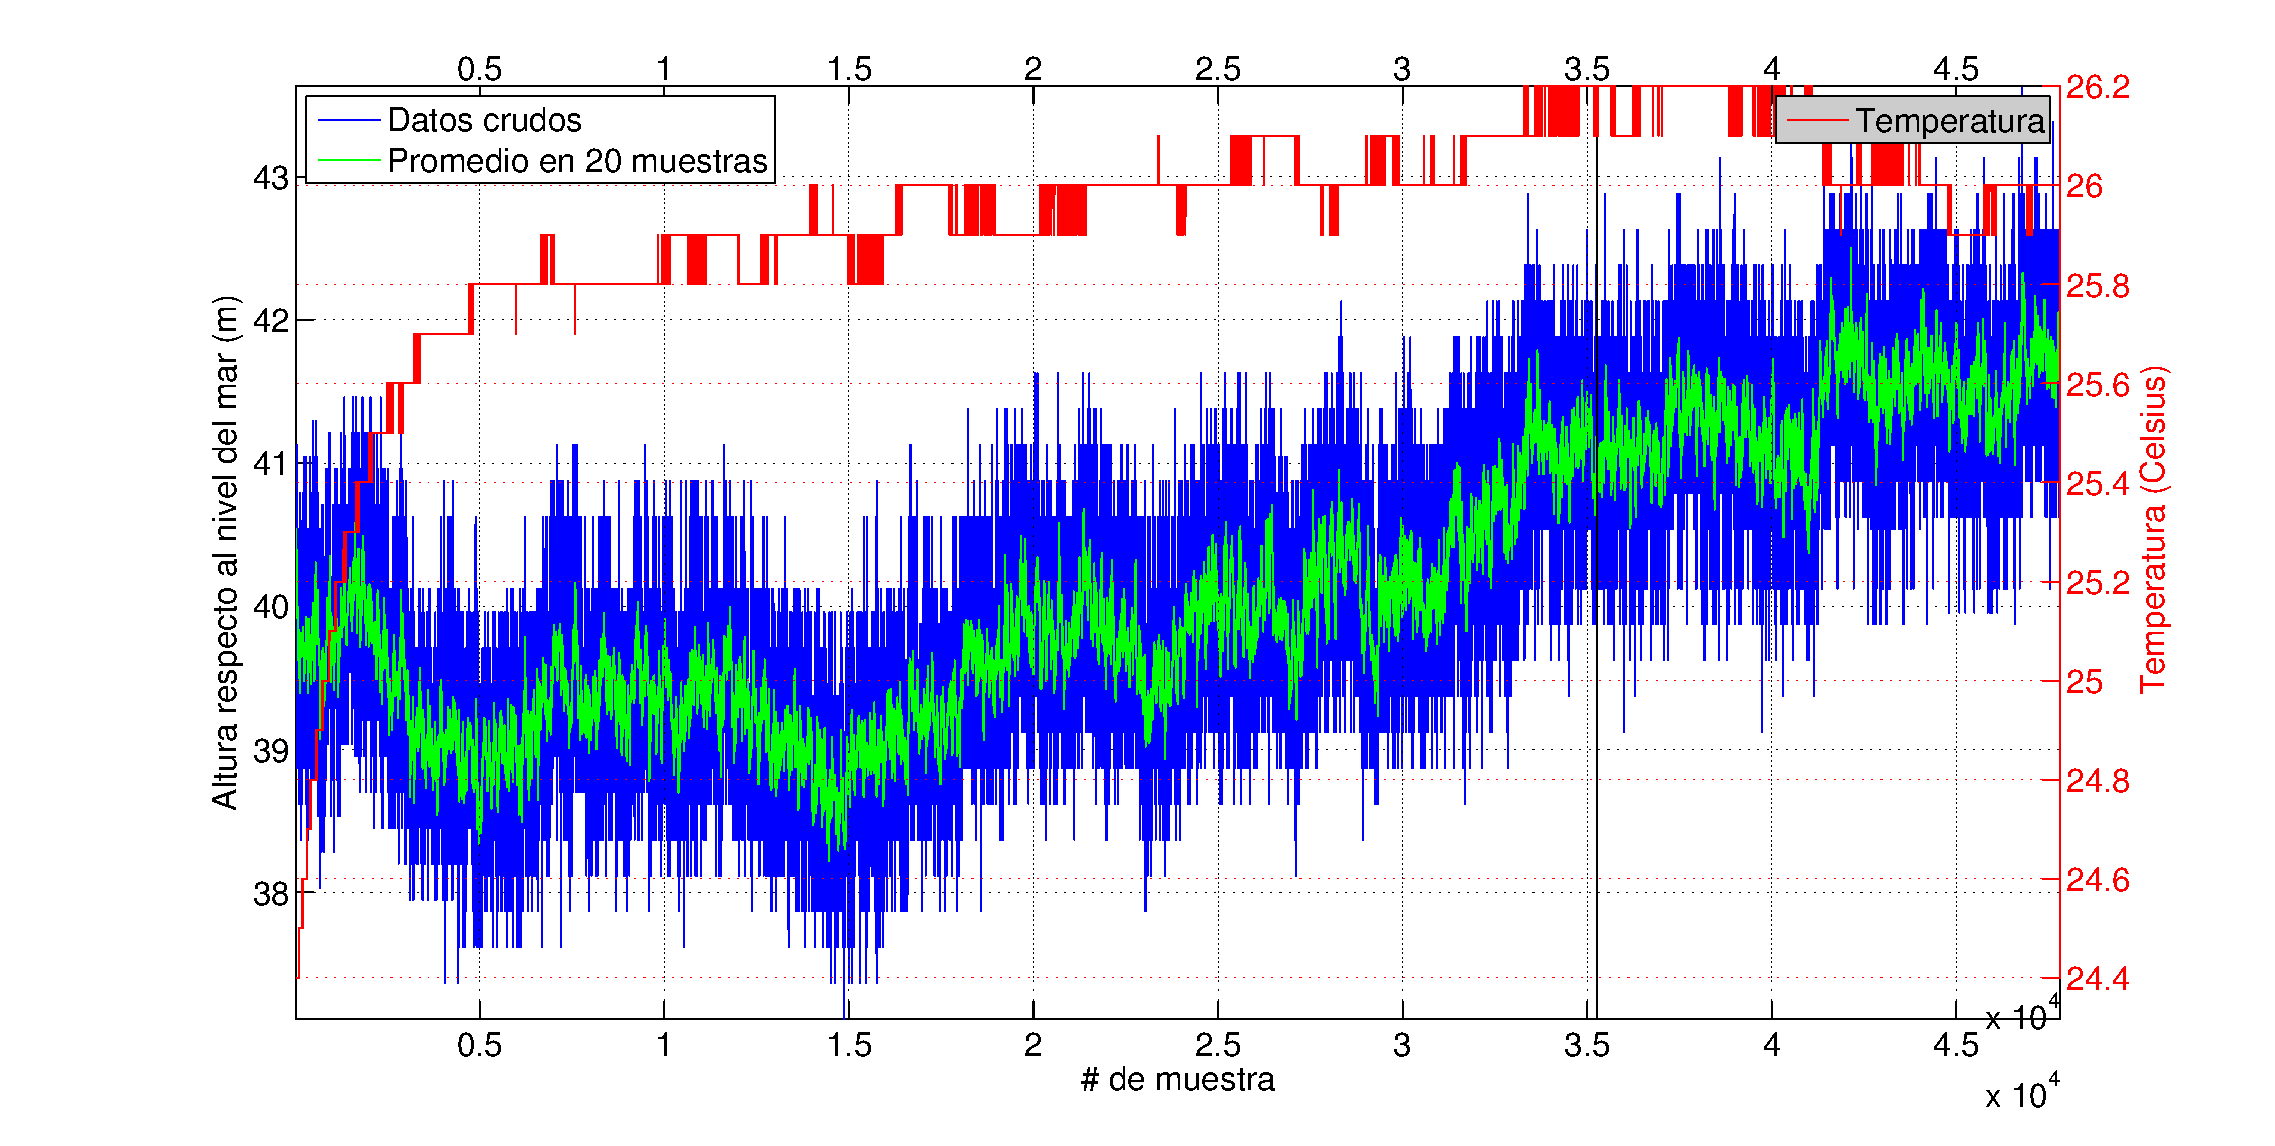
\includegraphics[width=.9\textwidth]{./pics/1hora_01.pdf}
  \caption{Muestras durante una hora, experimento \#1.}
  \label{fig:1hora_01.pdf}
\end{figure}

% \begin{figure}[h!]
%   \includegraphics[width=1\textwidth]{./pics/1hora_02.pdf}
%   \caption{Muestras durante una hora, experimento \#2.}
%   \label{fig:1hora_02.pdf}
% \end{figure}

Se observa que existe un tiempo de \textit{warm-up} bastante extenso, pero con un rango pequeño. La temperatura tarda entre 15 y 45 minutos en estabilizarse, y en el proceso varía menos de 2\degc. Las muestras del barómetro no parecen estar directamente correlacionadas con la temperatura.

El barómetro no parece ser adecuado para medir la elevación absoluta. En los datos de las figuras \ref{fig:1hora_01.pdf} y \ref{fig:1hora_04.pdf} se observan variaciones de hasta 3 metros en la estimación de la altura en un período de 1 hora. Sin embargo, el error en el corto plazo es significativamente menor, parece viable el uso del barómetro como estimador de la altura en el corto plazo. Esto se analiza más adelante.

\newpage
\subsection{Caracterización del ruido}
\label{sec:caract-ruido}

En los logs de la sección \ref{sec:drift-y-warm-up}, se observa que:
\begin{itemize}
\item El comportamiento del ruído en intervalos extensos no es estacionario.
\item La mayoría de los saltos en la medida de la altura son de aproximadamente 25cm, las especificaciones dan una resolución de 1Pa, que corresponden a una variación en altura de aproximadamente 8cm.
\end{itemize}

\subsubsection{Estacionaridad}

Analizando el ruído en intervalos más pequeños, donde el proceso se puede considerar estacionario, el comportamiento del ruído es muy similar al del ruído blanco.

En la figura \ref{fig:autocorr} se observa la autocorrelación de la muestras tomadas del barómetro en intervalos de tiempo de 5 minutos, 2 minutos, y 15 segundos.

Cabe destacar que el ruído se puede considerar estacionario si se usan intervalos de tiempo menores a 15 segundos.

\begin{figure}[H]
  \begin{center}
	\subfloat[Datos durante 5 minutos]{\label{fig:autocorr_5m.pdf}
	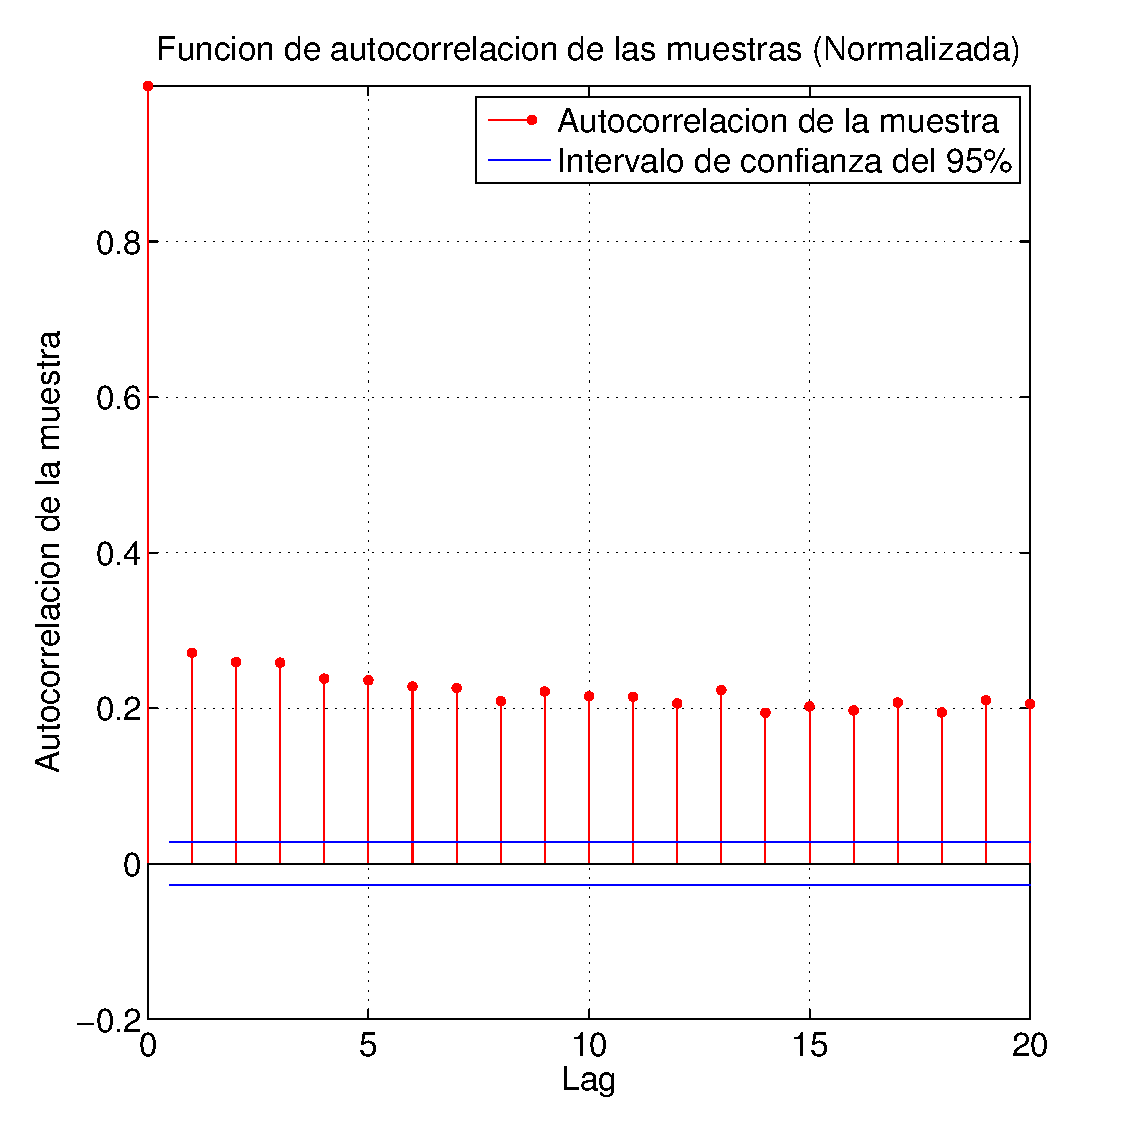
\includegraphics[width=0.4\textwidth]
		{./pics/autocorr_5m_log04.pdf}}
	\subfloat[Datos durante 15 segundos]{\label{autocorr_15s_log04.pdf}
	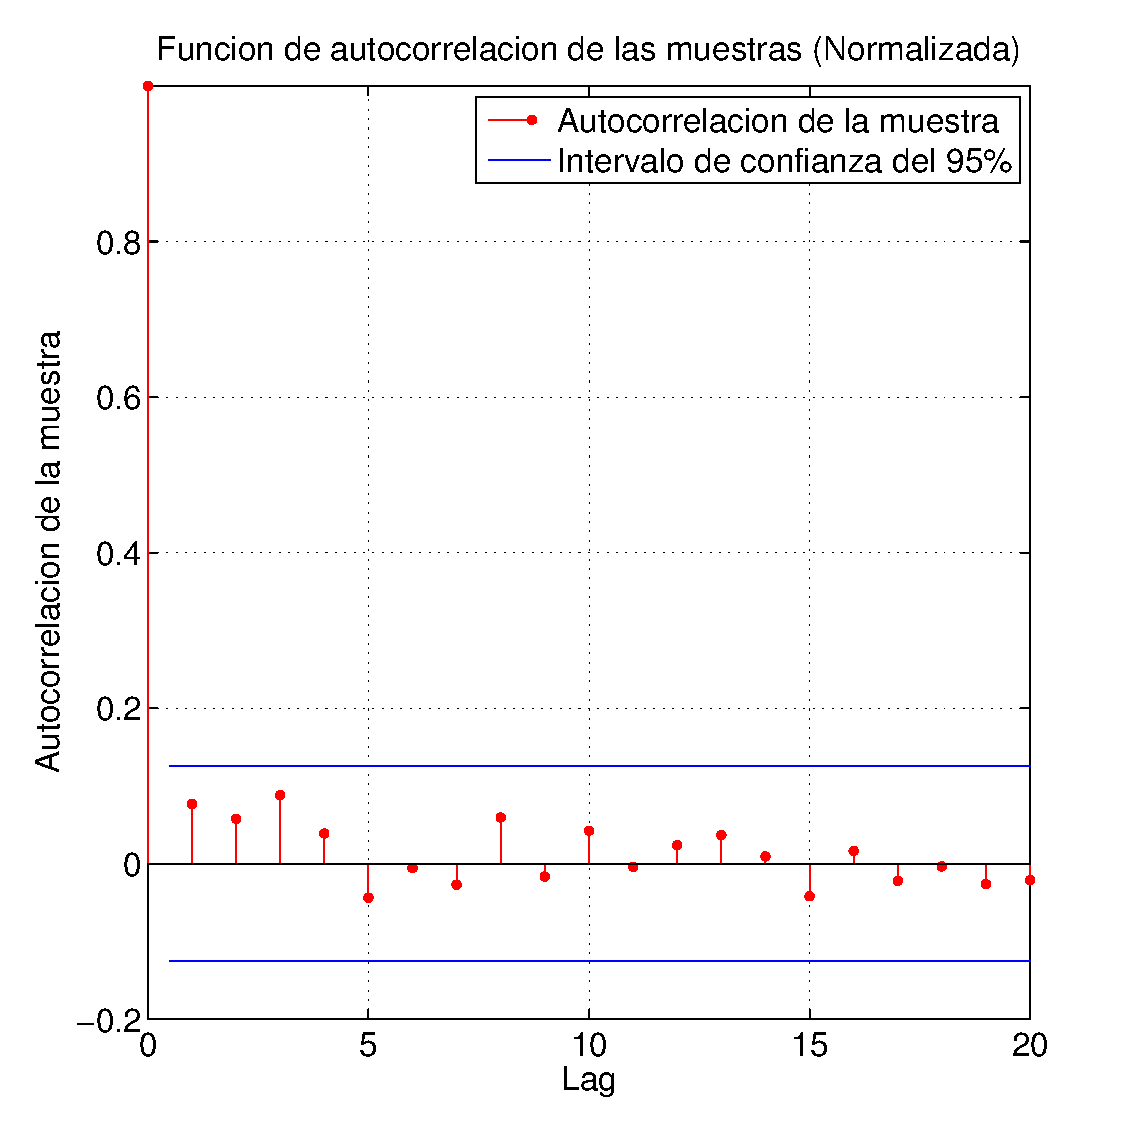
\includegraphics[width=0.4\textwidth]
		{./pics/autocorr_15s_log04.pdf}}\\
	\subfloat[Datos durante 15 segundos]{\label{autocorr_15s_log04.pdf}
	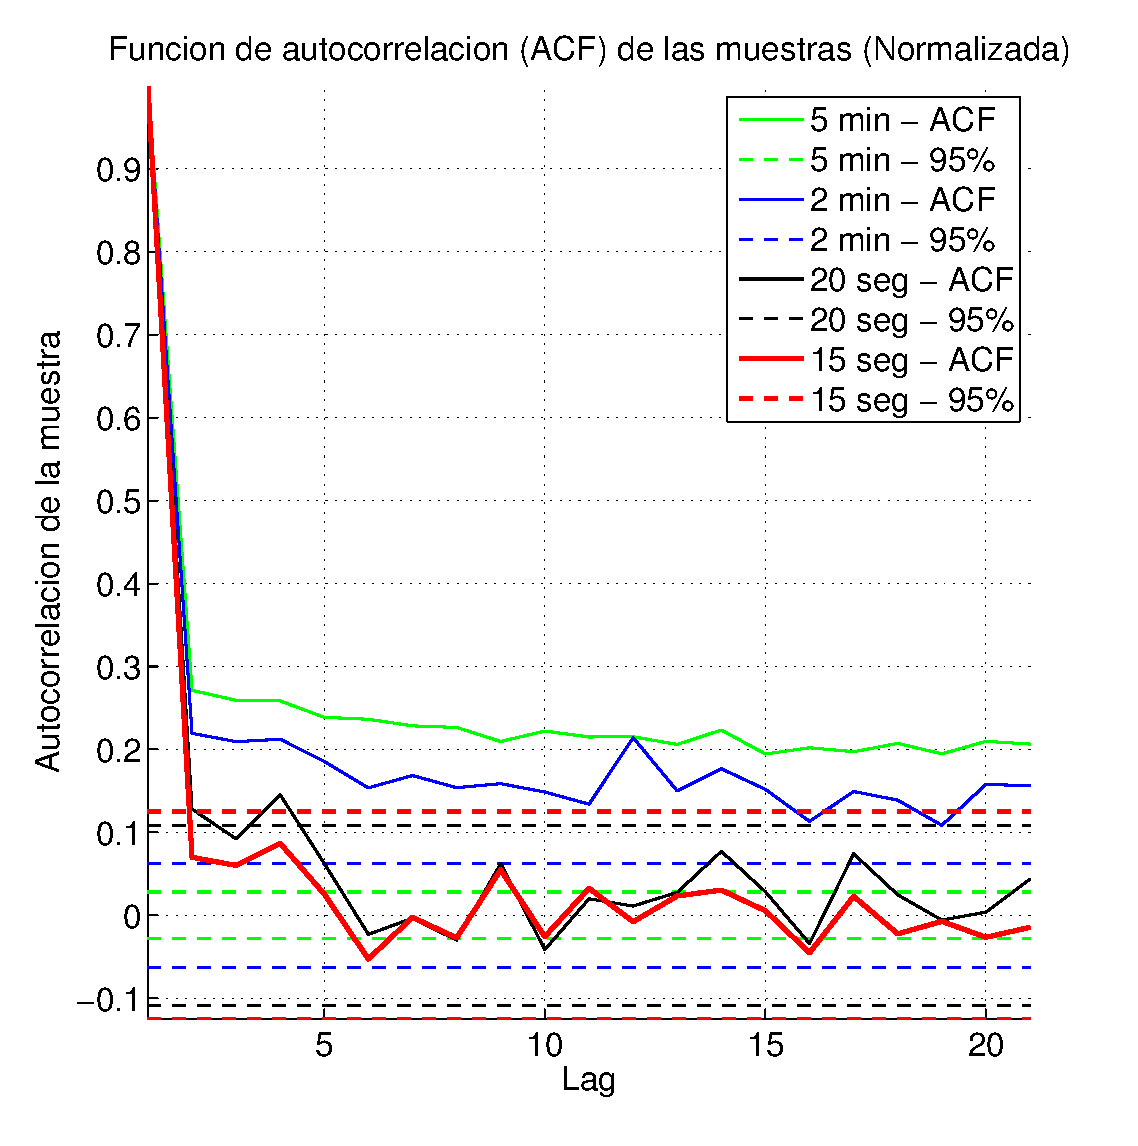
\includegraphics[width=.4\textwidth]
		{./pics/autocorr.pdf}}
  \end{center}
  \caption{Autocorrelación de las muestras del barómetros.}
\label{fig:autocorr}
\end{figure}

\subsubsection{Modos de funcionamiento}

El barómetro permite trabajar en varios modos. Basicamente, permite que se le exija más resolución, menos ruído, y a cambio aumenta el tiempo que tarda en tener un dato nuevo listo, y consume más energía. Esto lo logra promediando datos internamente. En la tabla \ref{tab:ruido-rms} se compara el ruído RMS en los distintos modos, con lo que se lograría usándolo en el modo básico (sin promediar internamente) y promediando en el microprocesador.

\begin{table}[H]
\centering
\begin{tabular}{c|c|c|c|} 
\cline{2-4}
	& \multicolumn{3}{|c|}{\cellcolor[gray]{0.8} Ruído RMS  (hPa)}      \\ \hline
\multicolumn{1}{|c|}{\cellcolor[gray]{0.8} {Modo}} & \cellcolor[gray]{0.8} {Computado} &\cellcolor[gray]{0.8} {Interno} &\cellcolor[gray]{0.8} {Specs}\\ \hline

\multicolumn{1}{|c|}{0}	&	0.52	&	0.52	&	0.50\\
\hline
\multicolumn{1}{|c|}{1}	&	0.37	&	0.45	&	0.40\\
\hline
\multicolumn{1}{|c|}{2}	&	0.25	&	0.37	&	0.30\\
\hline
\multicolumn{1}{|c|}{3}	&	0.63	&	0.35	&	0.25\\
\hline

\end{tabular}
\caption{Ruído RMS, 2 minutos de datos a 14Hz.}
\label{tab:ruido-rms}
\end{table}
\vspace{-15pt}
La resolución más atractiva parece ser la número 2, en la cual se promedian 4 datos. Se concluye que, si se dispone de procesador se optará por promediar datos en él, de lo contrario se usará el promedio calculado por el sensor.

\subsubsection{Resolución del instrumento}
En la figura \ref{fig:barom_hist_exp4.pdf} se observa un histograma de las diferencias entre muestras sucesivas de los datos del barómetro. Se observa que la mayor parte de los datos saltan de a 25cm. Se esperaba una discretización en niveles de  aproximadamente 8cm, correspondientes a variaciones de presión de 1Pa (la resolución del instrumento).

Puede resultar dificil ver que hay muestras en todos los bins, pero mirando con detalle se puede. Se descarta un problema de software en la adquisición de datos, y se atribuye el comportamiento al sensor en sí. Este problem no parece ser significativo.
\vspace{-15pt}
\begin{figure}[h!]
\centering
  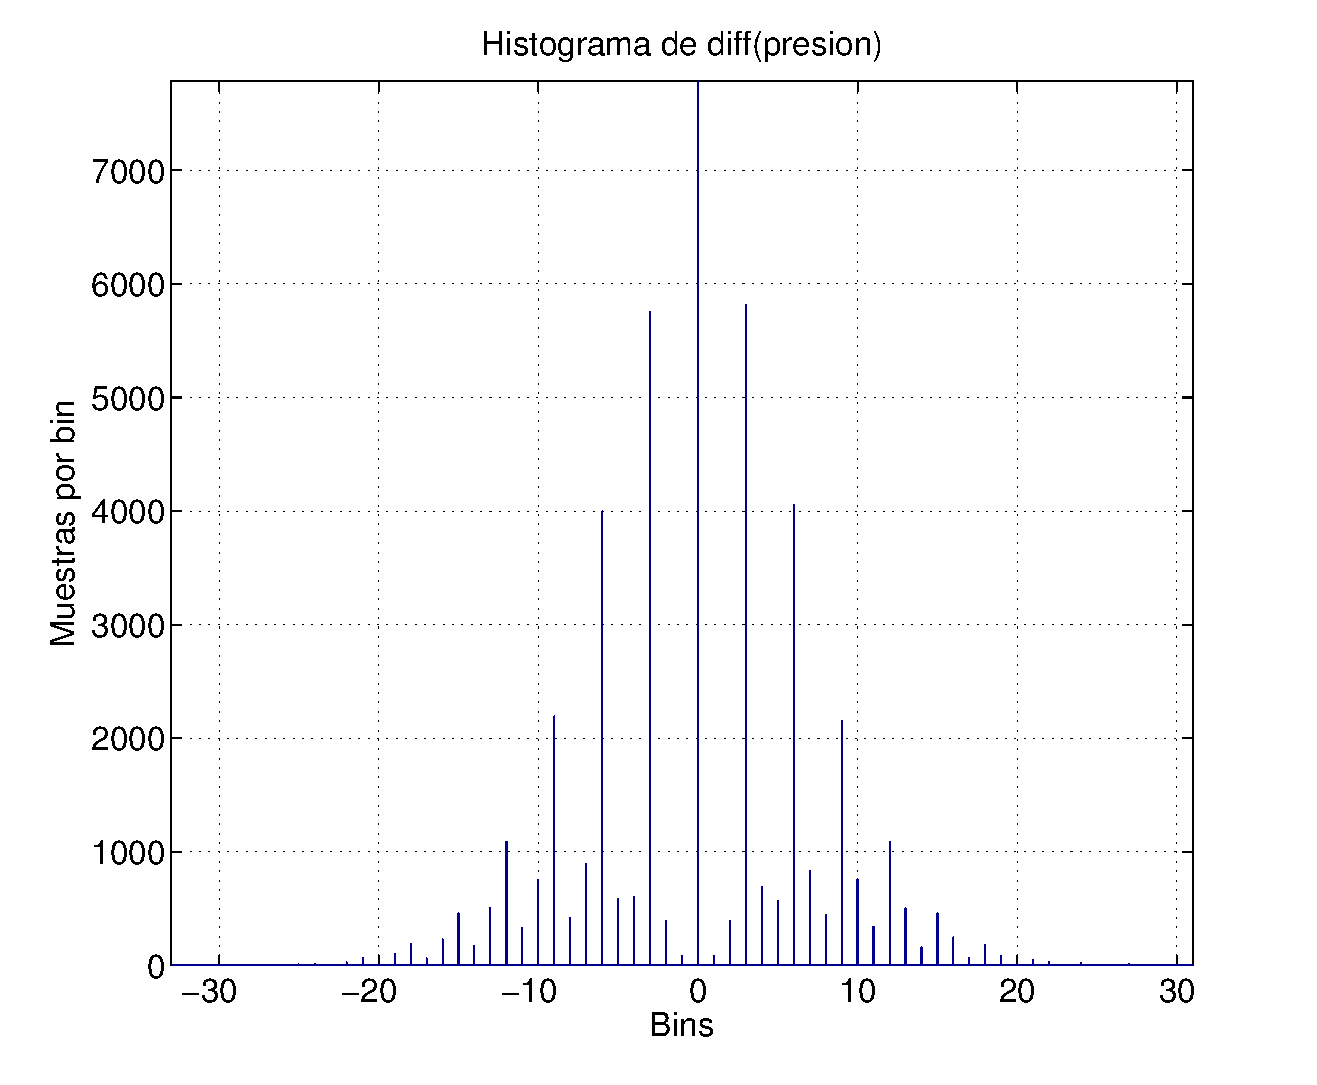
\includegraphics[width=.75\textwidth]{./pics/barom_hist_exp4.pdf}
\vspace{-15pt}
  \caption{Histograma de las diferencias, experimento \#4.}
  \label{fig:barom_hist_exp4.pdf}
\end{figure}
\vspace{-40pt}


\newpage
\subsection{Altura absoluta}

Las figuras \ref{fig:1hora_01.pdf} y \ref{fig:1hora_04.pdf} se corresponden a datos tomados a la misma altura, pero en dias distintos. Cabe destacar que la diferencia de los promedios es del orden de los 25 metros.

Se descartó la posibilidad de utilizar el barómetro para determinar la altura absoluta, ya que estando el barómetro a una altura fija, la elevación varía mucho de un dia a otro, lo cual refleja una fuerte dependencia con factores externos, probablemente climáticos.

\subsection{Distancias de varios metros}



\subsection{Distancias de un metro}

Las figuras \ref{fig:esc1.pdf} y \ref{fig:esc2.pdf} presentan las medidas obtenidas al realizar las medidas estáticas a alturas que difieren de un metro. La figura \ref{fig:variando} muestra las medidas obtenidas durante el proceso de subir y bajar el barómetro. En las tres figuras se observan los datos obtenidos y la media móvil considerando 20 muestras.

Se aprecia que el comportamiento es acorde a lo esperado, corresponde a las acciones realizadas. Analizaremos con mayor detenimiento los resultados para concluir que es lo que podemos esperar del barómetro.

\vspace{-25pt}
\begin{figure}[H]
\hspace{-70pt}
	\subfloat[Primer serie de medidas cada 1 metro.]{\label{fig:esc1.pdf}
  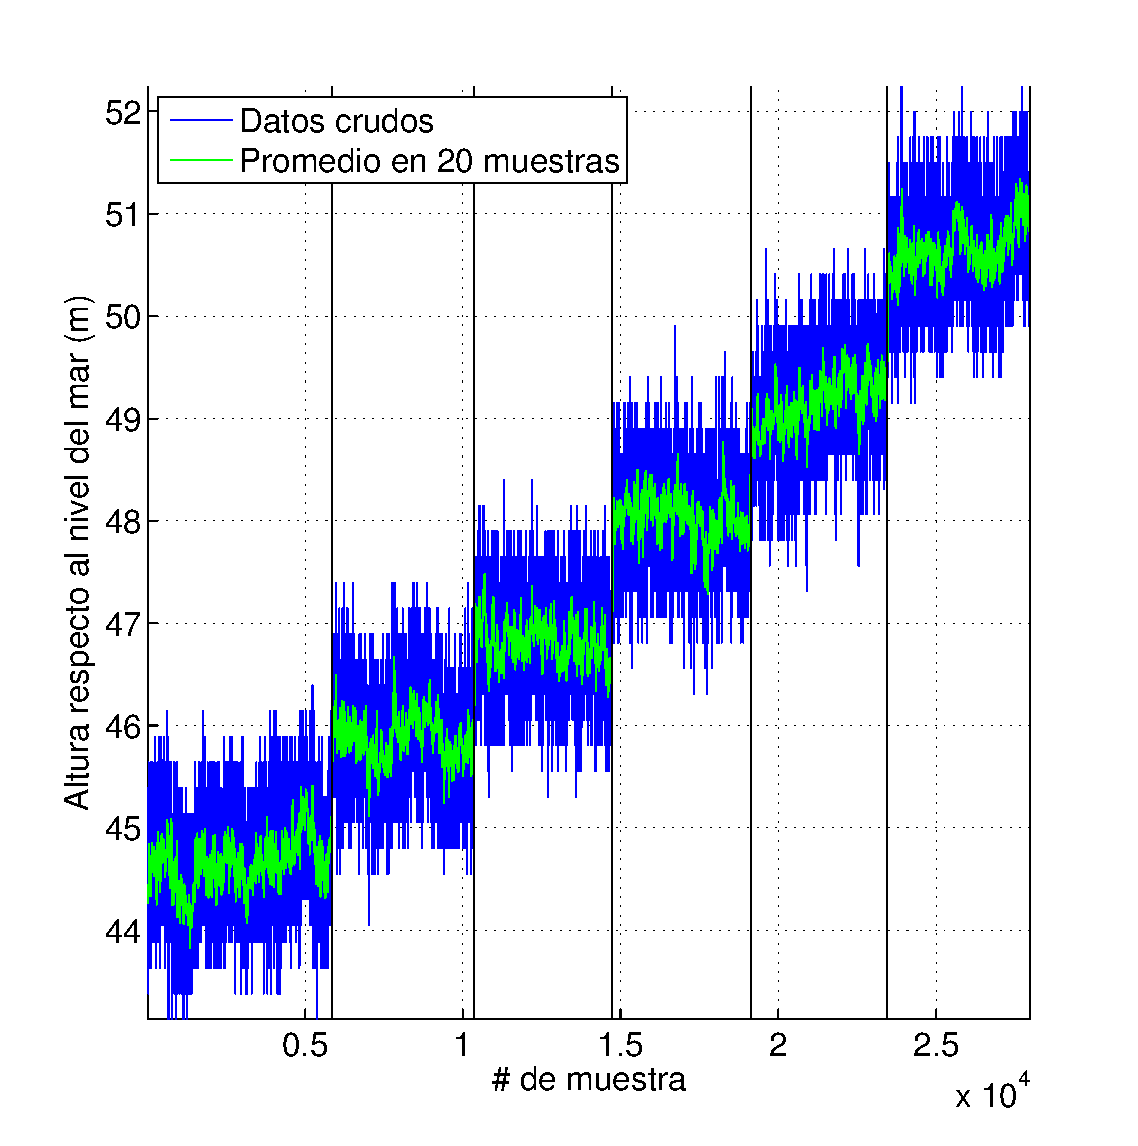
\includegraphics[width=.65\textwidth]{./pics/esc1.pdf}}
	\subfloat[Segunda serie de medidas cada 1 metro.]{\label{fig:esc2.pdf}
  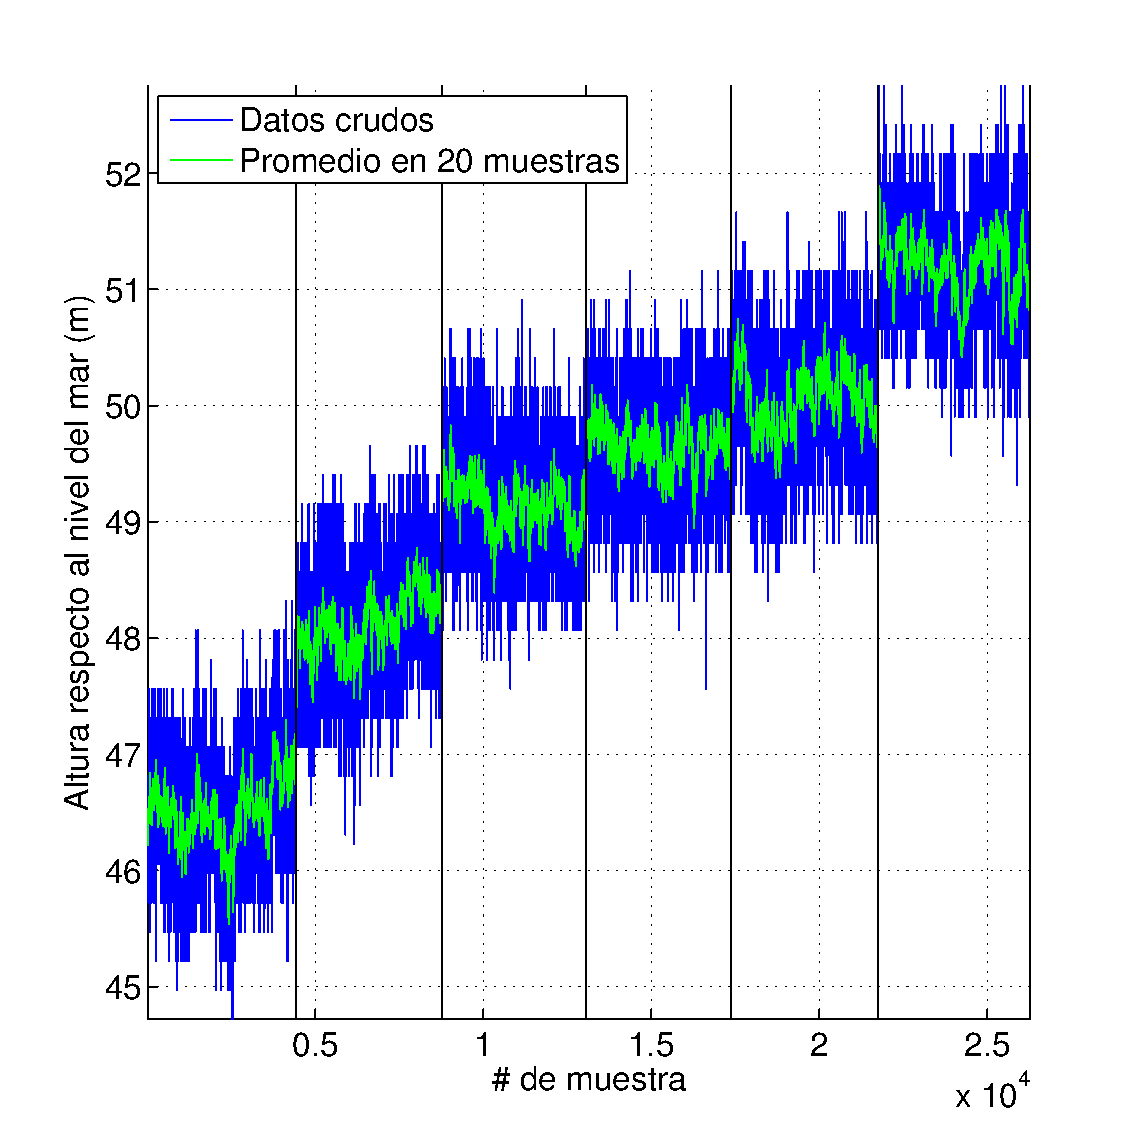
\includegraphics[width=.65\textwidth]{./pics/esc2.pdf}}
\vspace{-10pt}
  \caption{Experimento: Distancias de 1 metro.}
\label{fig:1m}
\end{figure}


%   \caption{}
%   \label{fig:esc2}
% \end{figure}

En la tabla \ref{tab:alturasm} se muestran los valores de altura obtenidos en las distintas posiciones en las dos series de datos tomadas. El valor absoluta de la altura no tiene sentido, ya que no se conoce la presión a nivel del mar en el momento de tomar las muestras.

\begin{table}[H]
\centering
\begin{tabular}{c|c|c|} 
	& \multicolumn{2}{|p{200pt}|}{\cellcolor[gray]{0.8} Altura medida con el barómetro (m)}      \\ \hline
\cellcolor[gray]{0.8} {Posición} & \cellcolor[gray]{0.8} {Serie 1} &\cellcolor[gray]{0.8} {Serie 2}\\ \hline

\multicolumn{1}{|c|}{1} & 44.66 & 46.52 \\ \hline
\multicolumn{1}{|c|}{2} & 45.87 & 48.12\\ \hline
\multicolumn{1}{|c|}{3} & 46.82 & 49.15\\ \hline
\multicolumn{1}{|c|}{4} & 48.04 & 49.66\\ \hline
\multicolumn{1}{|c|}{5} & 49.15 & 50.05\\ \hline
\multicolumn{1}{|c|}{6} & 50.66 & 51.21 \\ \hline

\end{tabular}
\caption{Alturas obtenidas con el barómetro}
\label{tab:alturasm}
\end{table}

Se observa inmediatamente en las medidas de altura realizadas que la altura absoluta registrada por el barómetro cambia considerablemente de una serie a la otra. En la segunda se observa que las medidas se encuentran en promedio un metro más arriba. Los puntos que se consideraron fueron los mismos, sin embargo las medidas fueron realizadas un día de tormenta. La presión atmosférica es muy cambiante en esos días. Eso puede explicar dicha diferencia. Otra explicación puede ser el drift observado en secciones previas.

El error RMS esperado es de 0.5m. En la figura \ref{fig:variando} se observa la variación en la altura absoluta. Si bien cada tramo comienza y termina a una altura que cae dentro del error esperado, el hay tramos del principio y el final del experimento, cuando el barómetro estaba en el suelo, en los que se observa una diferencia en altura de 1.5m, que no cae dentro del error esperado. El problema se ve luego de transcurridos varios minutos, tiempo mucho mayor al sugerido en la sección \ref{sec:caract-ruido}, por lo que no parece ser un problema relevante.

\begin{figure}[H]
\centering
  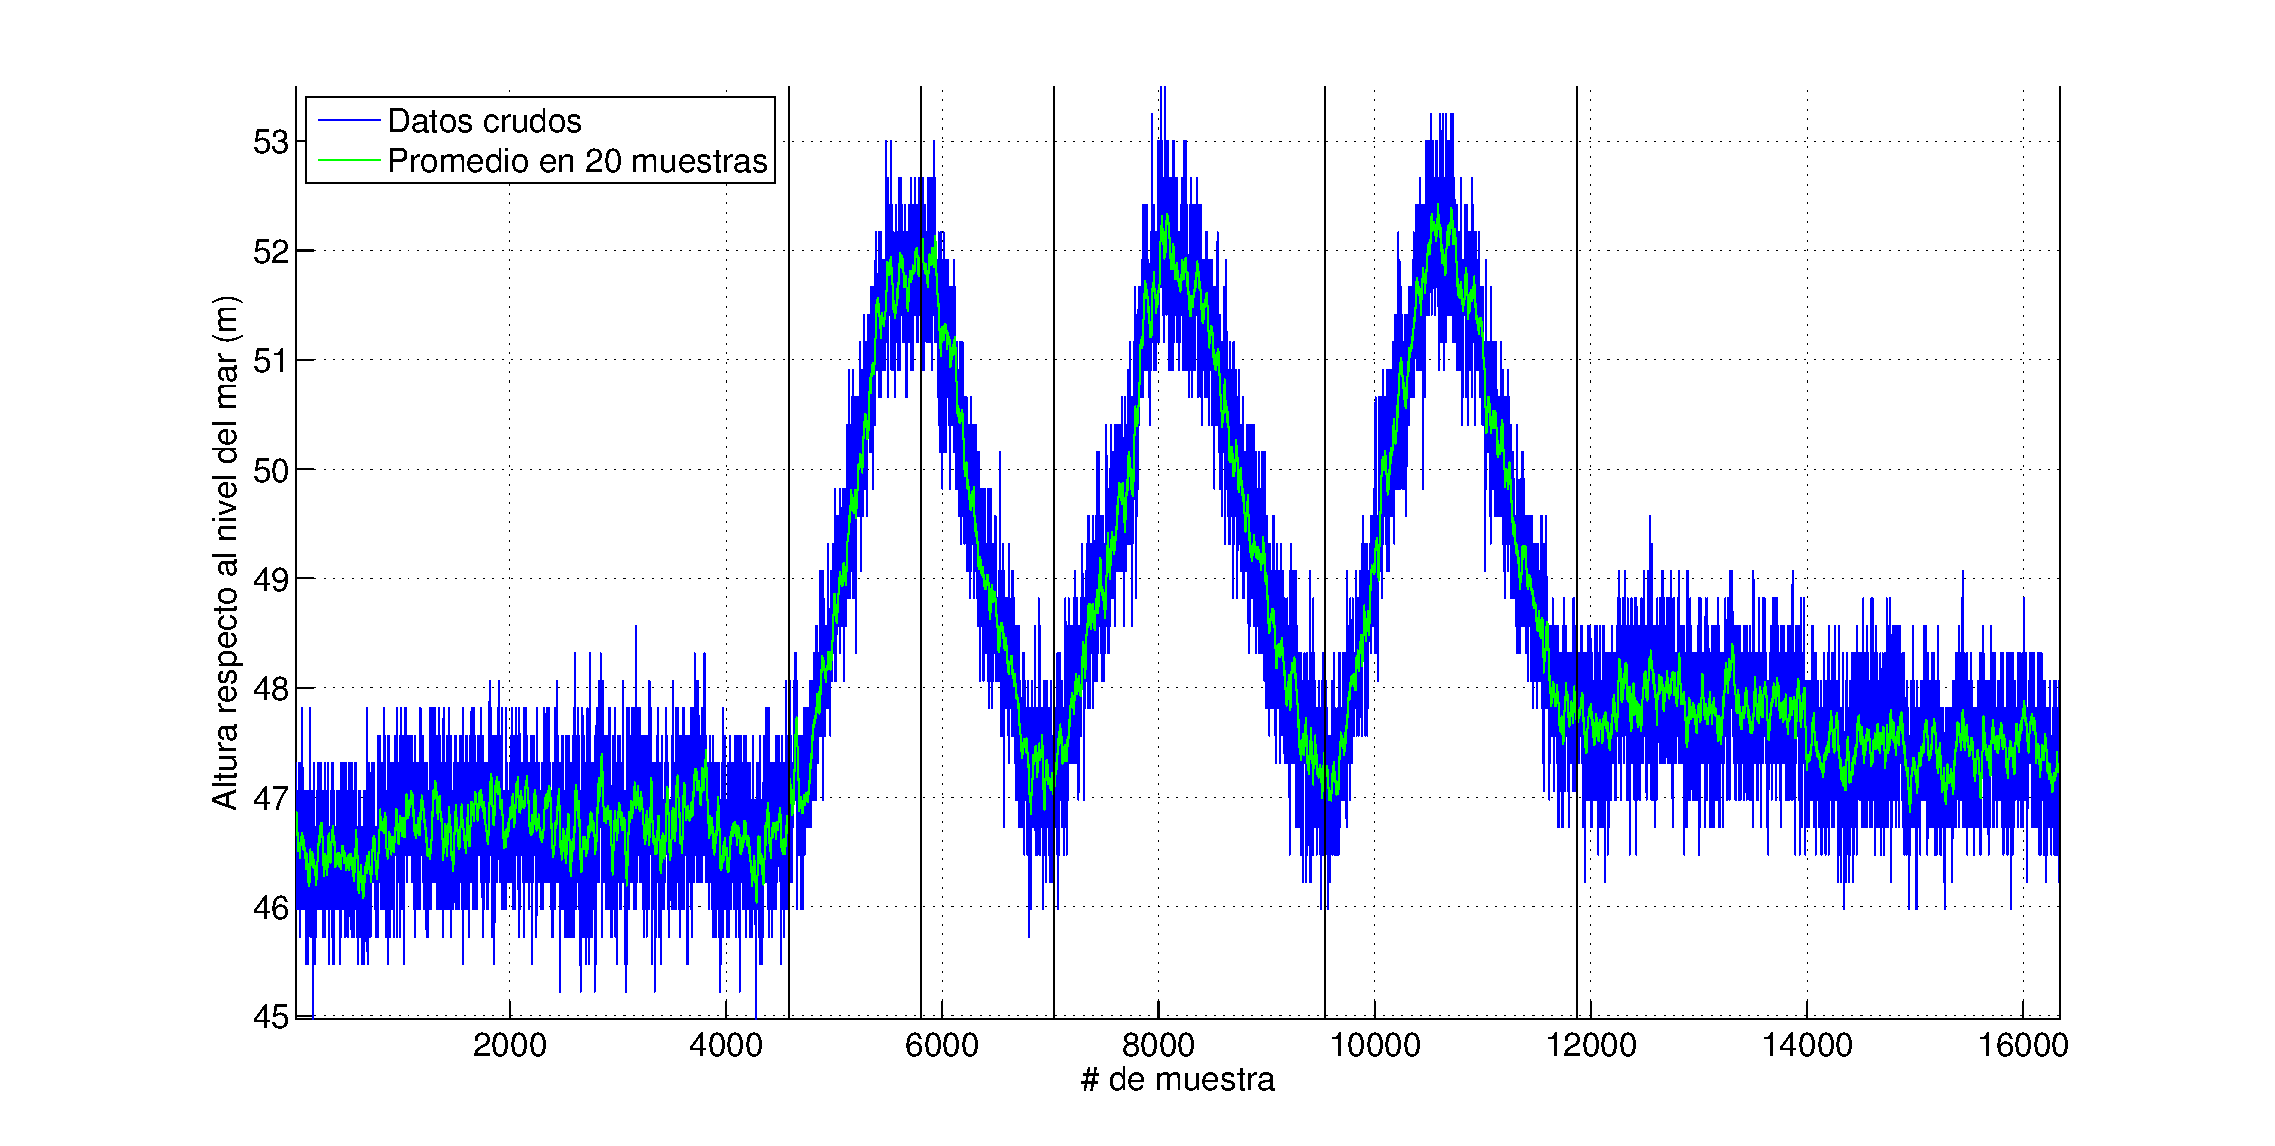
\includegraphics[width=1\textwidth]{./pics/variando.pdf}
  \caption{Medidas de altura subiendo y bajando.}
  \label{fig:variando}
\end{figure}

En cuanto al error promedio y a la desviación estándar se obtuvo para las dos series:

\begin{itemize}
\item Serie 1:
		\begin{itemize}
		\item Error promedio: $-0.20m$
		\item Desviación estándar: $0.20m$
		\end{itemize}
\item Serie 2:
		\begin{itemize}
		\item Error promedio: $0.06m$
		\item Desviación estándar: $0.49m$
		\end{itemize}
\end{itemize}

Al tener pocas muestras en cada una de las series es imposible considerarlas como buenas muestras estadísticas, de hecho ambas difieren mucho en cuanto al error promedio que presentan y la desviación estándar. 

Si trabajamos con las dos series de datos lo que obtenemos es:

\begin{itemize}
\item Error promedio: $-0.07m$
\item Desviación estándar: $0.38m$
\end{itemize}



A partir de los datos anteriores se puede concluir que el $95.5 \%$ de las veces tendremos errores inferiores a $0.76m$ en diferencias de un metro. Este error depende del drift del barómetro, y se puede reducir incorporando, de manera periódica, información externa (GPS) sobre la altura absoluta.

\subsection{Distancias de decenas de centímetros}

En la tabla \ref{tab:alturascm}


\begin{table}[H]
\centering
\begin{tabular}{|c|c|} 

	\cellcolor[gray]{0.8} {Altura medida con el barómetro(cm)} &
	\cellcolor[gray]{0.8} Altura medida con el metro (cm) \\ \hline
\end{tabular}
\caption{Alturas obtenidas con el metro y con el barómetro}
\label{tab:alturascm}
\end{table}


\newpage
\section{Conclusiones}
\label{sec:conclusiones}

La conclusiones más importante de las pruebas hechas con el barómetro fueron las siguientes:

\begin{itemize}
\item \textbf{Tiempo de \textit{warm-up}}: El circuito tiene un tiempo de \textit{warm-up} de aproximadamente 45 minutos, durante el cual la temperatura sube aproximadamente 1.5\degc. De las especificaciones de los sensores se deduce que una variación de temperatura tan pequeña no debería afectar la performance. De cualquier forma, es de interés analizar analizar, experimentalmente, el efecto de la variación de la temperatura sobre las lecturas de la IMU.
\item \textbf{Altura absoluta}: El drift y la sensibilidad a factores externos (clima, etc) hacen que el barómetro \textbf{no} sea adecuado para determinar la altura absoluta.
\item \textbf{Altura relativa}: La performance en períodos cortos de tiempo fue buena, es posible conocer variaciones de altura con una error menor a TODO, durante tiempo menores a TODO segundos/minutos.
\item \textbf{Rol del barómetro}: Se concluye que el barómetro servirá para determinar variaciones de altura, suavizando la trayectoria, mientras se espera una altura absoluta proveniente del GPS. El barómetro y el GPS se complementan.
\end{itemize}




\end{document}